
\section{Reference Implementation}

The reference implementation relies heavily upon the extensions that
are attached as part of the engine. Thus to see how the reference
implementation was designed we would refer to look at those extensions.

The extensions the reference implementation uses:
\begin{description}
\item [{Logger~Extension}] this is used to log all actions that occur
inside the engine and to log any errors that might also occur.
\item [{EIS~Extension}] this extension is used to connect the reference
implementation to our goal program for the agents inside the reference
implementation.
\item [{Tile~World~Extension}] the reference implementation uses a Tile
based world as such it directly uses the Tile World Extension that
provides just this functionality.
\end{description}
The reference implementation as such only provides:
\begin{itemize}
\item Actions specific to the reference implementation(Grabbing/releasing
packages)
\item Entities specific to the reference implementation(Walls, Player, etc.)
\item Percepts and modules specific to the reference implementation(Holding
package percept)
\item A view in console form
\item A Goal program
\item A way to control an agent with keyboard
\end{itemize}

\subsection{The Console View}

The console view is designed is optimized to draw the screen at a
specific frame rate. When the console view does not draw it will instead
update all view data is has stored.

To change view data in a view, an event must be fired from the model,
however since the model is operating on a different thread than the
view. The view must ensure no concurrent errors. This is done by using
the \texttt{ThreadSafeEventMananger}, as explained in \ref{ImplementationView}.

\begin{figure}
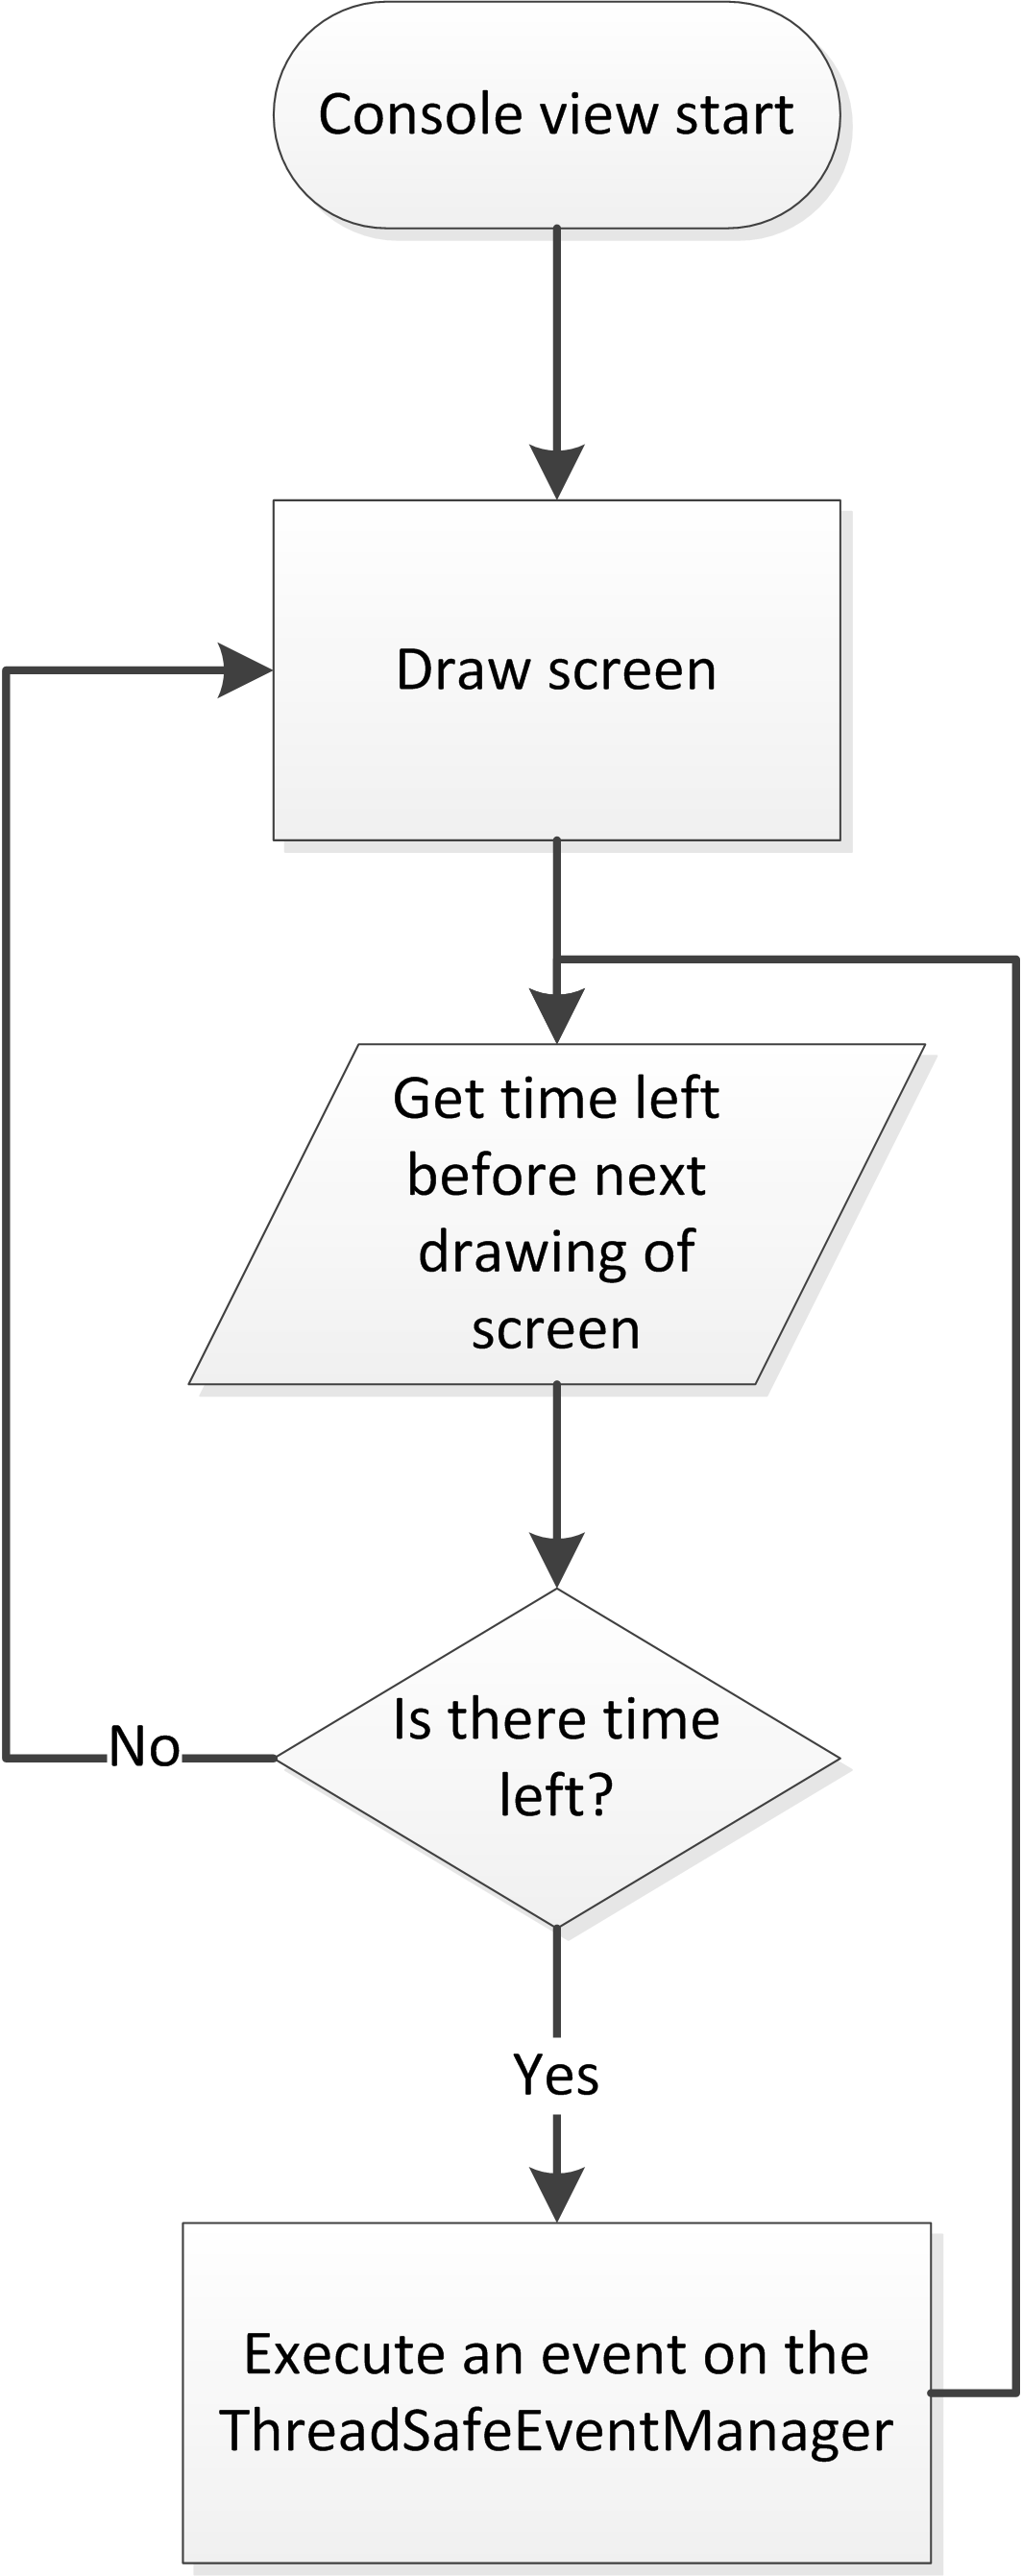
\includegraphics[width=0.4\textwidth]{ConsoleViewDrawingFlowChart}

\caption{the sequence of the console view drawing process\label{fig:FlowOfConsole}}


\end{figure}


The console view works by drawing the screen, then if it has time
between left before the next drawing is scheduled the view will execute
a single event on the \texttt{ThreadSafeEventManager}. The view will
continue this process until either, there is no events left to be
executed or the time is up and it is time for it to perform the next
drawing of the screen. On fig. \ref{fig:FlowOfConsole} a drawing
of this process can be seen.

This provides the reference implementation with a very quickly updated
view as no time is wasted on the thread and instead will continue
to update even when it is not drawing. Furthermore by updating the
view data in a separate thread the engine core does not use its computation
power on handling this making the engine overall more efficient.


\subsection{GOAL Program Implementation}

The goal program is designed to work directly with our reference implementation,
as it is just a show case of how such a program might look like, it
will make assumptions based on how the reference implementation interact.
For instance it will assume that there are entities called walls that
are meant to block off tiles. 

To see the source code of our goal program commented, look in appendix
\ref{GoalCodeAppendix}.


\subsubsection{Agent Decision}

A full flow chart of the goal program decision chart can be found
on appendix \ref{GOALFlowChartAppendix}.

As can be seen from the flow chart, the agent will try and find packages
and bring them to a dropzone, if no such packages can be found or
if no dropzone is found, the agent will start exploring the entire
world.

The goal program operates with a few different notions; 
\begin{description}
\item [{Street}] the first notion is the notion of streets. A tile is a
street if it contains no wall types such a normal walls or impassableWalls(map
boundary walls) this means that the agent can move on this tile.
\item [{Route}] all the agents decisions are preplanned this means that
the agent determines where to move to, this plan is put into a route,
the agent will follow this route whenever it has nothing else to do,
such as grabbing/releasing packages.
\end{description}
\begin{figure}
\begin{centering}
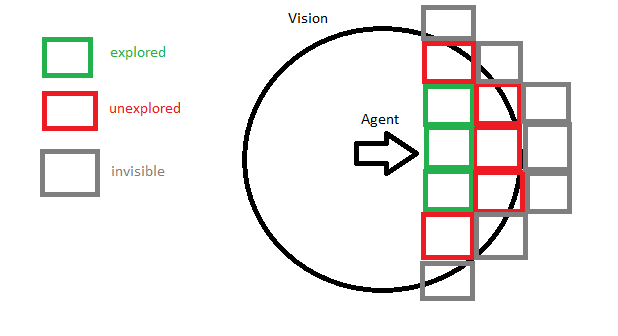
\includegraphics[width=0.8\textwidth]{VisionExploredGOALAgent}
\par\end{centering}

\caption{An image of an agent\textquoteright{}s vision and which it would determine
to be explored\label{fig:VisionExploredGoalAgent}}
\end{figure}

\begin{description}
\item [{Explored}] the agent\textquoteright{}s goal is to eventually have
all tiles explored as this means that all packages has been collected
from the world. The agent determines that a tile has been explored
if it has seen all its adjacent tiles. This works great for the agent
because until it reaches a wall the unexplored tiles that it has stored
as a street will always be considered unexplored, no matter how far
it moves, this makes the agent work much like putting a carrot in
front of a mule, no matter how much the agent explores whenever it
explores something, there is always something new that becomes unexplored.
As such this will continue until a wall has been reached on all its
paths. \\
A tile is determined to be explored if all tiles adjacent to has been
seen by the agent, fig. \ref{fig:VisionExploredGoalAgent} shows an
image of this.
\end{description}

\subsection*{Summary}

The reference implementation was designed as a reference for all the
features of the engine, as such it made heavily use of the extensions
that we implemented. This section only covered the view and the goal
program in details. This is because most of the reference implementation
consists of either declaring new agent/entity types or wiring all
the extensions together, as such there was almost no business logic
involved which makes them rather uninteresting to explain in detail.

One part that the reference implementation does not cover which could
have been interesting was the notion of linked module as explained
in \ref{SysFeatEntities}. This could have been used in the reference
implementation but we did not choose to do so.

Overall the design of the reference implementation is very solid and
fulfills the goals we had for it, which were to be a showcase for
our engine.
